
%=======================================================================
\chapter{Advanced Platform-Level Interrupt Controller (PLIC)}
\label{ch:AdvPLIC}
\chaptermark{Advanced PLIC}

\textbf{%
Warning!
This draft specification is likely to change before being accepted as
standard by the {\RISCV} International Association.%
}
\bigskip

In a {\RISCV} system, a Platform-Level Interrupt Controller (PLIC)
handles external interrupts that are signaled through wires rather than
by MSIs.
When the {\RISCV} harts in a system do not have IMSICs, the harts
themselves do not support MSIs, and all external interrupts to such
harts must pass through a PLIC.
But even in machines where harts have IMSICs and most interrupts are
communicated via MSIs, it is not unusual for some device interrupts
still to be signaled by dedicated wires.
In particular, for devices (or device controllers) that do not
otherwise need to be bus masters in the system, the cost of supporting
MSIs is especially high, so wired interrupts are a frugal alternative.
Wired interrupts also continue to be universally supported by all
current computer platforms, unlike MSIs, making another reason for many
commodity devices or controllers to choose wired interrupts over MSIs,
when not implementing a standard like PCI Express that dictates MSIs.

In a machine without IMSICs, every {\RISCV} hart accepts interrupts
from exactly one PLIC that is the \emph{external interrupt controller}
for that hart.
A hart's external interrupt controller (the PLIC) signals interrupts
to the hart through a dedicated connection, usually a wire, for each
privilege level that the hart may receive interrupts.
(Recall Figure~\ref{fig:intrsWithoutIMSICs} on
page~\pageref{fig:intrsWithoutIMSICs}.)
A system without IMSICs will typically have only one PLIC, serving as
the external interrupt controller for all {\RISCV} harts.

\begin{commentary}
Because every {\RISCV} hart without an IMSIC has exactly one PLIC
as its external interrupt controller, a system with multiple PLICs
must partition the harts into disjoint subsets, making each PLIC the
external interrupt controller for a separate subset of the harts.
While not prohibited, this arrangement is likely to be less efficient
than having all harts share a single PLIC.
\end{commentary}

{\RISCV} harts that employ IMSICs as their external interrupt
controllers can receive external interrupts only in the form of MSIs.
In that case, the role of a PLIC is to convert wired interrupts into
MSIs for harts.
(Recall Figure~\ref{fig:intrsWithIMSICs} on
page~\pageref{fig:intrsWithIMSICs}.)
The PLIC is said to \emph{forward} incoming wire-signaled interrupts to
harts by sending MSIs to the harts.

When harts have IMSICs to support MSIs, a system may easily contain
multiple PLICs for converting wired interrupts into MSIs, with each
PLIC forwarding interrupts from a different subset of devices.
Multiple PLICs are presumably more likely to arise when groups of
devices are physically distant from one another, perhaps even on
separate chips (including chiplets in a multi-chip module).

This chapter specifies an \emph{Advanced PLIC} that is not backward
compatible with the earlier {\RISCV} PLIC.
Full conformance to the Advanced Interrupt Architecture requires the
Advanced PLIC.
However, a workable system can be built substituting the older PLIC
instead, assuming only wired interrupts to harts, not MSIs.
Chapter~\ref{ch:DuoPLIC} describes a \emph{\mbox{Duo-PLIC\/}} that is
software-configurable to act as either an original {\RISCV} PLIC or an
Advanced PLIC.

\begin{commentary}
We intend eventually to provide a free example parameterized
implementation of an Advanced PLIC, written in portable SystemVerilog,
that we expect will be suitable for many {\RISCV} systems without
modification.
\end{commentary}

%-----------------------------------------------------------------------
\section{Interrupt sources and identities}

An individual PLIC supports a fixed number of \emph{interrupt sources},
corresponding exactly with the set of physical incoming interrupt
wires at the PLIC.
Most often, each source's incoming wire is connected to the output
interrupt wire from a single device or device controller.
(For level-sensitive interrupts, the interrupt outputs of multiple
devices or controllers may be combined to drive the incoming wire of a
single interrupt source at a PLIC.
An interrupt source's incoming wire might also be simply tied high or
low, if, for example, the source will always be configured as Detached.
See Section~\ref{sec:AdvPLIC-reg-sourcecfg} for a description of
\emph{source modes}.)

Each of a PLIC's interrupt sources has a fixed unique
\emph{identity number} in the range 1 to~$N$, where $N$ is the total
number of sources at the PLIC.
The number zero is not a valid interrupt identity number at a PLIC.
The maximum number of interrupt sources an Advanced PLIC may support is
1023.

When a PLIC delivers interrupts directly to harts at a given
privilege level (rather than forwarding interrupts as MSIs), the PLIC
is the external interrupt controller for the harts at that privilege
level, and the interrupt identities at the PLIC become directly the
\emph{minor identities} for external interrupts at the harts.

On the other hand, when a PLIC forwards interrupts by MSIs, software
configures a new interrupt identity number for the outgoing MSIs of
each source.
Consequently, in this case, the source identity numbers at a given
PLIC only distinguish the incoming interrupts at the PLIC and have no
relevance outside the PLIC.

%-----------------------------------------------------------------------
\section{Interrupt domains}

An Advanced PLIC supports one or more \emph{interrupt domains}, each
associated with a subset of {\RISCV} harts at one privilege level
(machine or supervisor level).
The harts within an interrupt domain are those that the domain can
interrupt at the corresponding privilege level.
Each domain has its own memory-mapped control region in the machine's
address space that appears to control a complete, separate PLIC,
though in fact all domain interfaces together access a single combined
interrupt controller.

Figures \ref{fig:AdvPLIC-ex-1Domain} through
\ref{fig:AdvPLIC-ex-3Domains} depict some possible hierarchies of
interrupt domains implemented by an Advanced PLIC in a {\RISCV} system.

The first figure represents a minimal system that has a single hart not
supporting supervisor mode, with a single interrupt domain for machine
level on that hart.
The next figure, \ref{fig:AdvPLIC-ex-2Domains}, shows a basic
arrangement for a larger system designed for symmetric multiprocessing
(SMP), with multiple harts that all implement supervisor mode.
In such cases, the PLIC will usually provide a separate interrupt
domain for supervisor level, as the figure portrays.
This supervisor-level interrupt domain allows an operating system,
running in \mbox{S-mode} on the multiple harts, to have direct control
over the interrupts it receives, avoiding the need to call upon
\mbox{M-mode} to exercise that control.

\begin{figure}[th]
\centerline{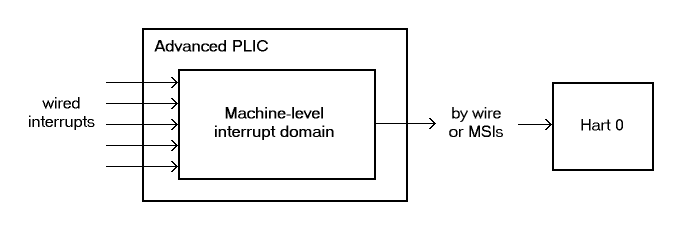
\includegraphics[scale=0.55]{AdvPLIC-ex-1Domain.png}}
\caption{%
Example of a {\RISCV} system that has a single hart implementing only
\mbox{M-mode}, with a single machine-level interrupt domain for that
hart.%
}
\label{fig:AdvPLIC-ex-1Domain}
\end{figure}

\begin{figure}[th]
\centerline{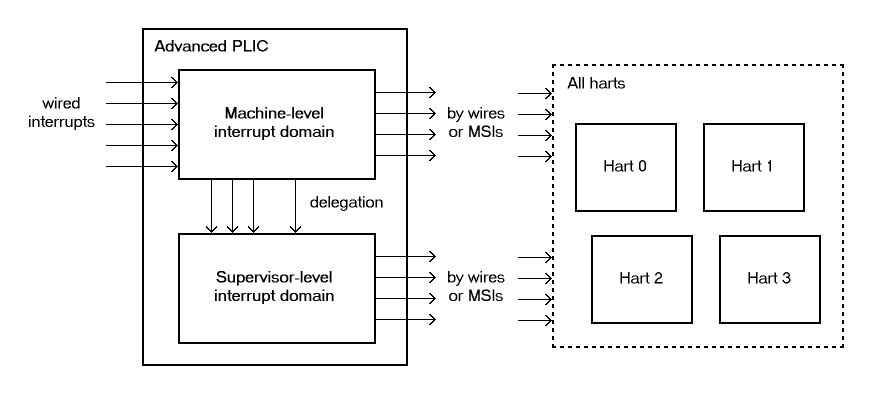
\includegraphics[scale=0.55]{AdvPLIC-ex-2Domains.png}}
\caption{%
An example system with four harts that implement \mbox{M-mode} and
\mbox{S-mode}, with two PLIC interrupt domains, one each for machine
and supervisor levels.%
}
\label{fig:AdvPLIC-ex-2Domains}
\end{figure}

A PLIC's interrupt domains are arranged in a tree hierarchy, with the
root domain always being at machine level.
Incoming interrupt wires arrive first at the root domain.
Each domain may then selectively delegate all or a subset of interrupt
sources to its child domains in the hierarchy.
Within a given PLIC, interrupt source numbers are invariant across all
domains, so source identity number~$i$ always refers to the same source
in every domain, corresponding to incoming wire number~$i$.
For an interrupt domain below the root, interrupt sources not delegated
down to that domain appear to the domain as being not implemented.

Figure~\ref{fig:AdvPLIC-ex-3Domains} shows a hierarchy of three
interrupt domains, two at machine level and one at supervisor level.
The arrangement in the figure, when combined with PMP (physical memory
protection), allows machine-level software to isolate a selection
of interrupts exclusively for hart~0, beyond the reach of the four
application harts, even at machine level.

\begin{figure}[th]
\centerline{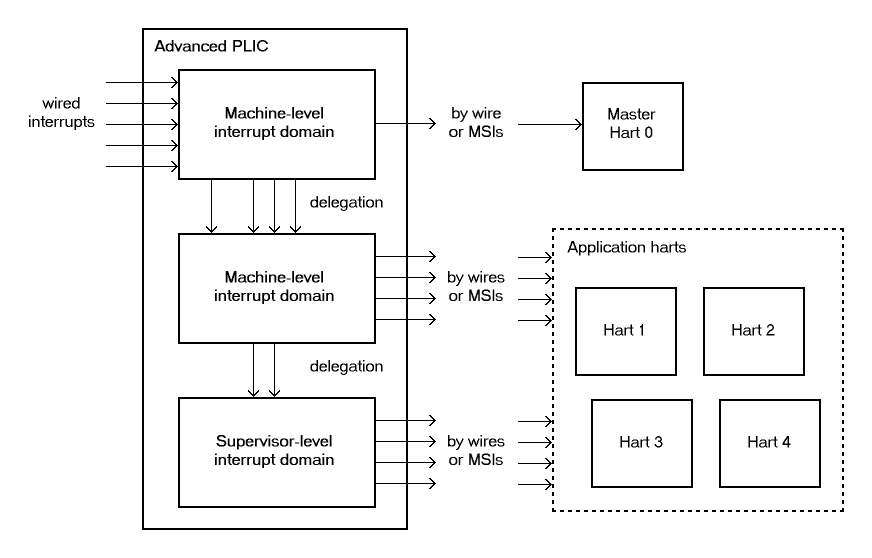
\includegraphics[scale=0.55]{AdvPLIC-ex-3Domains.png}}
\caption{%
A {\RISCV} system that extends the example of
Figure~\ref{fig:AdvPLIC-ex-2Domains} with a fifth \mbox{M-mode}-only
``master'' hart, with a separate machine-level interrupt domain above
the other domains.%
}
\label{fig:AdvPLIC-ex-3Domains}
\end{figure}

%*** REMOVE?:
\FloatBarrier

\begin{commentary}
In order for the harts within an interrupt domain to have direct
control over the interrupts from the domain, the harts must be
cooperatively controlled by software at the same privilege level.
In particular, a single operating system should control all of the
harts associated with a supervisor-level interrupt domain.
In the examples of Figures \ref{fig:AdvPLIC-ex-2Domains}
and~\ref{fig:AdvPLIC-ex-3Domains}, control of the PLIC's
supervisor-level interrupt domain could not be safely split among
multiple independent OSes.

Given the domain hierarchies depicted in the figures, if it were
necessary to partition the application harts for multiple OSes,
machine-level software would need to prevent direct OS access to the
supervisor-level interrupt domain and instead provide SBI services
for controlling PLIC interrupts or, alternatively, emulate the control
interfaces of separate superivsor-level interrupt domains, one for each
OS.
Note that such emulation might still make use of the PLIC's
physical supervisor-level interrupt domain, but under the control of
machine-level software.
\end{commentary}

A PLIC's interrupt domain hierarchy satisfies these rules:
\begin{itemize}

\item
The root domain is at machine level.

\item
The parent of any supervisor-level interrupt domain is a machine-level
domain that includes at least the same harts (but at machine level,
obviously).
The parent domain may have a larger set of harts at machine level.

\item
For each interrupt domain, interrupts from the domain are signaled
to harts all by the same method, either by wire or by MSIs, not by a
mixture of methods among the harts.

\end{itemize}

When a {\RISCV} hart's external interrupt controller is a PLIC, not an
IMSIC, the hart can be within only one interrupt domain of this PLIC at
each privilege level.

On the other hand, a hart that has an IMSIC for its external interrupt
controller may, at each privilege level, be in multiple PLIC interrupt
domains, even those of the same PLIC, and may potentially receive MSIs
from multiple different PLICs in the machine.

A platform might give software a way to choose between multiple
interrupt domain hierarchies for any given PLIC.
Any such configurability is outside the scope of this specification,
but should be available to machine level only.

%-----------------------------------------------------------------------
\section{Hart index numbers}

Within a given interrupt domain, each of the domain's harts has a
unique \emph{index number} in the range 0 to ${\mbox{2}^{14}-\mbox{1}}$
(=~16,383).
The index number a domain associates with a hart may or may not have
any relationship to the unique hart identifier (``hart ID'') that the
{\RISCV} Privileged Architecture assigns to the hart.
Two different interrupt domains may employ entirely different index
numbers for the same set of harts.
However, if any of a PLIC's interrupt domains can forward interrupts by
MSI, then all machine-level domains of the PLIC share a common mapping
of index numbers to harts.

\begin{commentary}
For efficiency, implementations should prefer small integers for hart
index numbers.
\end{commentary}

%-----------------------------------------------------------------------
\section{Overview of interrupt control for a single domain}

Each interrupt domain implemented by a PLIC has its own separate
physical control interface that is memory-mapped in the machine's
address space, allowing access to each domain to be easily regulated
by both PMP (physical memory protection) and page-based address
translation.
The control interfaces of all interrupt domains have a common
structure.
In most respects, every domain appears to software as though it were
a root domain, without visibility of the domains above it in the
hierarchy.

An individual interrupt domain has the following components for each
interrupt source at the PLIC:
\begin{itemize}

\item
Source configuration.
This determines whether the specific source is active in the domain
and, if so, how the incoming wire is to be interpreted, such as
level-sensitive or edge-sensitive.
For a source that is inactive in the domain, source configuration
controls any delegation to a child domain.

\item
Interrupt-pending and interrupt-enable bits.
For an inactive source, these two bits are read-only zeros.
Otherwise, the pending bit records an interrupt that arrived and has
not yet been signaled or forwarded, while the enable bit determines
whether interrupts from this source should currently be delivered, or
should remain pending.

\item
Target selection.
For an active source, target selection determines the hart to receive
the interrupt and either the interrupt's priority or the new interrupt
identity when forwarding as an MSI.

\end{itemize}

For interrupt domains that deliver interrupts directly to harts rather
than forwarding by MSIs, the domain has a final set of components for
controlling interrupt delivery to harts, one instance per hart in the
domain.

\begin{commentary}
Although a PLIC with multiple interrupt domains may appear to duplicate
the per-source state listed above (source configuration, etc.) by a
factor equal to the number of domains, in fact, PLIC implementations
can exploit the fact that each source is ultimately active in only one
domain.
In all domains to which a specific interrupt source has not been
delegated, the state associated with the source appears as read-only
zeros, requiring no physical register bits.
\end{commentary}

%-----------------------------------------------------------------------
\section{Memory-mapped control region for an interrupt domain}
\label{sec:AdvPLIC-domainControlRegion}

For each interrupt domain that a PLIC supports, there is a dedicated
memory-mapped control region for managing interrupts in that domain.
This control region is a multiple of 4~KiB in size and aligned to a
\mbox{4-KiB} address boundary.
The smallest valid control region is 16~KiB.
An interrupt domain's control region is populated by a set of
\mbox{32-bit} registers.
The first 16~KiB contains the registers listed in
Table~\ref{tab:AdvPLIC-domainControlRegion}.

\begin{table*}[p]
\begin{center}
\begin{tabular}{c@{\quad\ }l@{\qquad}ll}
\multicolumn{1}{l}{offset} & \ size & register name \\
\noalign{\medskip}
\z{0x0000} & 4 bytes & \z{domaincfg} \\
\z{0x0004} & 4 bytes & \z{sourcecfg[}1\z{]} \\
\z{0x0008} & 4 bytes & \z{sourcecfg[}2\z{]} \\
\dots      &         & \ \dots \\
\z{0x0FFC} & 4 bytes & \z{sourcecfg[}1023\z{]} \\
\z{0x1BC0} & 4 bytes & \z{mmsiaddrcfg}  & (machine-level interrupt domains only) \\
\z{0x1BC4} & 4 bytes & \z{mmsiaddrcfgh} & \quad '' \\
\z{0x1BC8} & 4 bytes & \z{smsiaddrcfg}  & \quad '' \\
\z{0x1BCC} & 4 bytes & \z{smsiaddrcfgh} & \quad '' \\
\z{0x1C00} & 4 bytes & \z{setip[}0\z{]} \\
\z{0x1C04} & 4 bytes & \z{setip[}1\z{]} \\
\dots      &         & \ \dots \\
\z{0x1C7C} & 4 bytes & \z{setip[}31\z{]} \\
\z{0x1CDC} & 4 bytes & \z{setipnum} \\
\z{0x1D00} & 4 bytes & \z{in\_clrip[}0\z{]} \\
\z{0x1D04} & 4 bytes & \z{in\_clrip[}1\z{]} \\
\dots      &         & \ \dots \\
\z{0x1D7C} & 4 bytes & \z{in\_clrip[}31\z{]} \\
\z{0x1DDC} & 4 bytes & \z{clripnum} \\
\z{0x1E00} & 4 bytes & \z{setie[}0\z{]} \\
\z{0x1E04} & 4 bytes & \z{setie[}1\z{]} \\
\dots      &         & \ \dots \\
\z{0x1E7C} & 4 bytes & \z{setie[}31\z{]} \\
\z{0x1EDC} & 4 bytes & \z{setienum} \\
\z{0x1F00} & 4 bytes & \z{clrie[}0\z{]} \\
\z{0x1F04} & 4 bytes & \z{clrie[}1\z{]} \\
\dots      &         & \ \dots \\
\z{0x1F7C} & 4 bytes & \z{clrie[}31\z{]} \\
\z{0x1FDC} & 4 bytes & \z{clrienum} \\
\z{0x2000} & 4 bytes & \z{setipnum\_le} \\
\z{0x2004} & 4 bytes & \z{setipnum\_be} \\
\z{0x3000} & 4 bytes & \z{genmsi} \\
\z{0x3004} & 4 bytes & \z{target[}1\z{]} \\
\z{0x3008} & 4 bytes & \z{target[}2\z{]} \\
\dots      &         & \ \dots \\
\z{0x3FFC} & 4 bytes & \z{target[}1023\z{]} \\
\end{tabular}
\end{center}
\bigskip
\caption{%
The registers of the first 16~KiB of an interrupt domain's memory-mapped
control region.%
}
\label{tab:AdvPLIC-domainControlRegion}
\end{table*}

Starting at offset \z{0x4000}, an interrupt domain's control region
may optionally have an array of \emph{interrupt delivery control} (IDC)
structures, one for each potential hart index number in the range 0 to
some maximum that is at least as large as the maximum hart index number
for the interrupt domain.
IDC structures are used only when the domain is configured to deliver
interrupts directly to harts instead of being forwarded by MSIs.
An interrupt domain that supports only interrupt forwarding by MSIs
and not the direct delivery of interrupts by the PLIC does not need IDC
structures in its control region.

The first IDC structure, if any, is for the hart with index number~0;
the second is for the hart with index number~1; and so forth.
Each IDC structure is 32~bytes and has these defined registers:
\begin{displayLinesTable}[c@{\quad\ }l@{\qquad}l]
offset   & \ size  & register name \\
\noalign{\medskip}
\z{0x00} & 4 bytes & \z{idelivery} \\
\z{0x04} & 4 bytes & \z{iforce} \\
\z{0x08} & 4 bytes & \z{ithreshold} \\
\z{0x18} & 4 bytes & \z{topi} \\
\z{0x1C} & 4 bytes & \z{claimi} \\
\end{displayLinesTable}
IDC structures are packed contiguously, 32~bytes per structure, so the
offset from the beginning of an interrupt domain's control region to
its second IDC structure (hart index~1), if it exists, is \z{0x4020};
the offset to the third IDC structure (hart index~2), if it exists, is
\z{0x4040}; etc.

The array of IDC structures may include some for \emph{potential} hart
index numbers that are not \emph{actual} hart index numbers in the
domain.
For example, the first IDC structure is always for hart index~0, but 0
is not necessarily a valid index number for any hart in the domain.
For each IDC structure in the array that does not correspond to a valid
hart index number in the domain, the IDC structure's registers may
(or may not) be all read-only zeros.

Aside from the registers in Table~\ref{tab:AdvPLIC-domainControlRegion}
and those listed above for IDC structures, all other bytes in an
interrupt domain's control region are reserved and are implemented as
read-only zeros.

Only naturally aligned \mbox{32-bit} simple reads and writes are
supported within an interrupt domain's control region.
Writes to read-only bytes are ignored.
For other forms of accesses (other sizes, misaligned accesses, or
AMOs), implementations should preferably report an access fault or
bus error but must otherwise ignore the access.

The registers of the first 16~KiB of an interrupt domain's control
region (all but the IDC structures) are documented individually below.
IDC structures are documented later, in
Section~\ref{sec:AdvPLIC-directMode},
``Interrupt delivery directly by the PLIC.''

%- - - - - - - - - - - - - - - - - - - - - - - - - - - - - - - - - - - -
\subsection{Domain configuration (\zSafe{domaincfg})}

The \z{domaincfg} register has this format:\nopagebreak
\begin{displayLinesTable}[l@{\quad}l]
bits 31:24 & read-only \z{0x80} \\
bit 8      & IE \\
bit 7      & read-only 0 \\
bit 2      & DM (\WARL) \\
bit 0      & BE (\WARL) \\
\end{displayLinesTable}
All other register bits are reserved and read as zeros.

Bit IE (Interrupt Enable) is a global enable for all active interrupt
sources at this interrupt domain.
Only when IE~=~1 are pending-and-enabled interrupts actually signaled
or forwarded to harts.

Field DM (Delivery Mode) is {\WARL} and determines how this interrupt
domain delivers interrupts to harts.
The two possible values for DM are:
\begin{displayLinesTable}
0~=~direct delivery mode\\
1~=~MSI delivery mode\\
\end{displayLinesTable}
In \emph{direct delivery mode}, interrupts are prioritized and signaled
directly to harts by the PLIC itself.
In \emph{MSI delivery mode}, interrupts are forwarded by the PLIC
as MSIs to harts, presumably for further handling by IMSICs at those
harts.
A given PLIC implementation may support either or both of these
delivery modes for each interrupt domain.

If the interrupt domain's harts have IMSICs, the relevant interrupt
files of those IMSICs must support value \z{0x40000000} for register
\z{eidelivery}, else setting DM to zero (direct delivery mode) will
always have the same effect as setting IE to zero.
See Sections \ref{sec:IMSIC-reg-eidelivery}
and~\ref{sec:AdvPLIC-directMode-intrDelivery}.

BE (Big-Endian) is a {\WARL} field that determines the byte order for
most registers in the interrupt domain's memory-mapped control region.
If BE~=~0, byte order is little-endian, and if BE~=~1, it is
big-endian.
For {\RISCV} systems that support only little-endian, BE may be
read-only zero, and for those that support only big-endian, BE may be
read-only one.
For bi-endian systems, BE is writable.

Field BE affects the byte order of accesses to the \z{domaincfg}
register itself, just as for other registers in the interrupt domain's
control region.
To deal with this fact, the read-only value in \z{domaincfg}'s
most-significant byte, bits 31:24, serves two purposes.
First, for any read of \z{domaincfg}, the register's correct byte order
is easily determined from the four-byte value obtained:
When interpreted in the correct byte order, bit~31 is one, and in the
wrong order, bit~31 is zero.
Second, if the value of BE is uncertain (prior to software
initializing the interrupt domain, presumably), an \mbox{8-bit}
value~$x$ can be safely written to \z{domaincfg} by writing
\mbox{($x$\,\z{<<}\,24) \z{|} $x$}, where \mbox{\z{<<}\,24} represents
shifting left by 24~bits, and the vertical bar (\z{|}) represents
bitwise logical OR.
After \z{domaincfg} is written once, the value of BE should then be
known, so subsequent writes should not need to repeat the same trick.

At system reset, all writable bits in \z{domaincfg} are initialized to
zero, including~IE.
If an implementation supports additional forms of reset for the PLIC,
it is implementation-defined (or possibly platform-defined) how these
other resets may affect \z{domaincfg}.

%- - - - - - - - - - - - - - - - - - - - - - - - - - - - - - - - - - - -
\subsection{%
Source configurations
 (\zSafe{sourcecfg[{\rm 1}]}--\zSafe{sourcecfg[{\rm 1023}]})%
}
\label{sec:AdvPLIC-reg-sourcecfg}

For each possible interrupt source~$i$, register \z{sourcecfg[$i$]}
controls the \emph{source mode} for source~$i$ in this interrupt domain
as well as any delegation of the source to a child domain.
When source~$i$ is not implemented, or appears in this domain not to be
implemented, \z{sourcecfg[$i$]} is read-only zero.
If source~$i$ was not delegated to this domain and is then
changed (at the parent domain) to become delegated to this domain,
\z{sourcecfg[$i$]} remains zero until successfully written with a
nonzero value.

Bit~10 of \z{sourcecfg[$i$]} is a \mbox{1-bit} field called~D
(Delegate).
If D~=~1, source~$i$ is delegated to a child domain, and if D~=~0, it
is not delegated to a child domain.
Interpretation of the rest of \z{sourcecfg[$i$]} depends on field~D.

When interrupt source~$i$ is delegated to a child domain,
\z{sourcecfg[$i$]} has this format:\nopagebreak
\begin{displayLinesTable}[l@{\qquad}l]
bit 10   & D, = 1 \\
bits 9:0 & Child Index (\WLRL) \\
\end{displayLinesTable}
All other register bits are reserved and read as zeros.

Child Index is a {\WLRL} field that specifies the interrupt domain to
which this source is delegated.
For an interrupt domain with $C$~child domains, this field must be able
to hold integer values in the range 0 to ${C-\mbox{1}}$.
Each interrupt domain has a fixed mapping from these index numbers to
child domains.

If an interrupt domain has no children in the domain hierarchy, bit~D
cannot be set to one in any \z{sourcecfg} register for that domain.
For such a leaf domain, attempting to write a \z{sourcecfg} register
with a value that has bit~10 =~1 causes the entire register to be set
to zero instead.

When interrupt source~$i$ is not delegated to a child domain,
\z{sourcecfg[$i$]} has this format:\nopagebreak
\begin{displayLinesTable}[l@{\qquad}l]
bit 10   & D, = 0 \\
bits 2:0 & SM (\WARL) \\
\end{displayLinesTable}
All other register bits are reserved and read as zeros.

The SM (Source Mode) field is {\WARL} and controls whether the
interrupt source is active in this domain, and if so, what values or
transitions on the incoming wire are interpreted as interrupts.
The values allowed for SM and their meanings are listed in
Table~\ref{tab:AdvPLIC-sourcecfg-SM}.
Inactive (zero) is always supported for field~SM.
Implementations are free to choose, independently for each interrupt
source, what other values are supported for SM.

\begin{table*}[h!]
\begin{center}
\begin{tabular}{|c|c|l|}
\hline
Value & Name   & Description \\
\hline
\hline
0    & Inactive & Inactive in this domain (and not delegated) \\
1    & Detached & Active, detached from the source wire \\
2--3 & ---      & \emph{Reserved} \\
4    & Edge1    & Active, edge-sensitive; interrupt asserted on rising edge \\
5    & Edge0    & Active, edge-sensitive; interrupt asserted on falling edge \\
6    & Level1   & Active, level-sensitive; interrupt asserted when high \\
7    & Level0   & Active, level-sensitive; interrupt asserted when low \\
\hline
\end{tabular}
\end{center}
\caption{%
Encoding of the SM (Source Mode) field of a \z{sourcecfg} register when
bit~D =~0%
}
\label{tab:AdvPLIC-sourcecfg-SM}
\end{table*}

An interrupt source is inactive in the interrupt domain if either the
source is delegated to a child domain (D~=~1) or it is not delegated
(D~=~0) and SM is Inactive.
Whenever interrupt source~$i$ is inactive in an interrupt domain,
the corresponding interrupt-pending and interrupt-enable bits within
the domain are read-only zeros, and register \z{target[$i$]} is also
read-only zero.
If source~$i$ is changed from inactive to an active mode, the
interrupt source's pending and enable bits remain zeros, unless set
automatically for a reason specified later in this section or in
Section~\ref{sec:AdvPLIC-pendingBits}, and \z{target[$i$]} becomes an
{\unspecified} valid value.

When a source is configured as Detached, its wire input is ignored;
however, the interrupt-pending bit may still be set by a write to a
\z{setip} or \z{setipnum} register.
(This mode can be useful for receiving MSIs, for example.)

An edge-sensitive source can be configured to recognize an incoming
interrupt on either a rising edge (low-to-high transition) or a falling
edge (high-to-low transition).
When configured for a falling edge (mode Edge0), the source is said to
be \emph{inverted}.

A level-sensitive source can be configured to interpret either a
high level~(1) or a low level~(0) on the wire as the assertion of an
interrupt.
When configured for a low level (mode Level0), the source is said to be
\emph{inverted}.

For an interrupt source that is configured as edge-sensitive or
level-sensitive, define\nopagebreak
\begin{displayLinesTable}
\emph{rectified input value} = (incoming wire value) XOR (source is inverted).
\end{displayLinesTable}
For a source that is inactive or Detached, the
\emph{rectified input value} is zero.

Any write to a \z{sourcecfg} register might (or might not) cause the
corresponding interrupt-pending bit to be set to one if the rectified
input value is high (=~1) under the new source mode.
A write to a \z{sourcecfg} register will not by itself cause a pending
bit to be cleared except when the source is made inactive.
(But see Section~\ref{sec:AdvPLIC-pendingBits}.)

%- - - - - - - - - - - - - - - - - - - - - - - - - - - - - - - - - - - -
\subsection{%
Machine MSI address configuration
 (\zSafe{mmsiaddrcfg} and \zSafe{mmsiaddrcfgh})%
}
\label{sec:AdvPLIC-reg-mmsiaddrcfg}

For machine-level interrupt domains, registers \z{mmsiaddrcfg}
and \z{mmsiaddrcfgh} may optionally provide parameters used to
determine the addresses to write outgoing MSIs.

If no interrupt domain of the PLIC supports MSI delivery
mode (\z{domaincfg}.DM is read-only zero for all domains),
these two registers are not implemented for any domain.
Otherwise, they are implemented for the root domain, and may
or may not be implemented for other machine-level domains.
For domains not at machine level, they are never implemented.
When a domain does not implement \z{mmsiaddrcfg} and
\z{mmsiaddrcfgh}, the eight bytes at their locations
are simply read-only zeros like other reserved bytes.

Registers \z{mmsiaddrcfg} and \z{mmsiaddrcfgh} are
potentially writable only for the root domain.
For all other machine-level domains that implement them,
they are read-only.

When implemented, \z{mmsiaddrcfg} has this format:\nopagebreak
\begin{displayLinesTable}[l@{\quad}l]
bits 31:0 & Low Base PPN (\WARL) \\
\end{displayLinesTable}
and \z{mmsiaddrcfgh} has this format:\nopagebreak
\begin{displayLinesTable}[l@{\quad}l]
bit 31     & L \\
bits 28:24 & HHXS (\WARL) \\
bits 22:20 & LHXS (\WARL) \\
bits 18:16 & HHXW (\WARL) \\
bits 15:12 & LHXW (\WARL) \\
bits 11:0  & High Base PPN (\WARL) \\
\end{displayLinesTable}
All other bits of \z{mmsiaddrcfgh} are reserved and read as zeros.

Fields High Base PPN from \z{mmsiaddrcfgh} and Low Base PPN from
\z{mmsiaddrcfg} concatenate to form a \mbox{44-bit} Base PPN
(Physical Page Number).
The use of this value and fields HHXS (High Hart Index Shift),
LHXS (Low Hart Index Shift), HHXW (High Hart Index Width),
and LHXW (Low Hart Index Width) for
determining target addresses for MSIs is described later, in
Section~\ref{sec:AdvPLIC-MSIAddrs}.

When \z{mmsiaddrcfg} and \z{mmsiaddrcfgh} are writable
(root domain only), all fields other than L are {\WARL}.
An implementation is free to choose what values are supported.
Typically, some bits are writable while others are read-only constants.
In the extreme, the values of all fields may be entirely
constant, fixed by the implementation.

If bit~L in \z{mmsiaddrcfgh} is set to one, \z{mmsiaddrcfg} and
\z{mmsiaddrcfgh} are \emph{locked}, and writes to the registers are
ignored, making the registers effectively read-only.
When L~=~1, the other fields in \z{mmsiaddrcfg} and \z{mmsiaddrcfgh}
may optionally all read as zeros.
In that case, if these other fields were given nonzero values
when L was first set in the root domain,
their values are retained internally by the
PLIC but become no longer visible by reading \z{mmsiaddrcfg} and
\z{mmsiaddrcfgh}.

Setting \z{mmsiaddrcfgh}.L to one also locks registers
\z{smsiaddrcfg} and \z{smsiaddrcfgh} described in the next
subsection, if those registers are implemented as well.

For the root domain, L~is initialized at
system reset to either zero or one, whichever is
deemed appropriate for the specific PLIC implementation.
If reset initializes L to one, either the other fields are
hardwired by the PLIC to constants, or the PLIC has a different means,
outside of this standard, for determining the addresses of outgoing MSI
writes.
In the latter case, the other fields in \z{mmsiaddrcfg} and
\z{mmsiaddrcfgh} may all read as zeros, so registers \z{mmsiaddrcfg} and
\z{mmsiaddrcfgh} have only read-only values zero and \z{0x80000000}
respectively.
Any time \z{mmsiaddrcfg} or \z{mmsiaddrcfgh} has a different value
(not zero or \z{0x80000000} respectively), the addresses for
outgoing MSI writes directed to machine level must be derivable
from the visible values of these registers, as specified in
Section~\ref{sec:AdvPLIC-MSIAddrs}.

For machine-level domains that are not the root domain, if these
registers are implemented, bit~L is always one, and the other
fields either are read-only copies of \z{mmsiaddrcfg} and
\z{mmsiaddrcfgh} from the root domain, or are all zeros.

\begin{commentary}
Giving software the ability to arbitrarily determine the addresses to
which MSIs are sent, even if allowed only for machine level, permits
bypassing physical memory protection (PMP).
For PLICs that support MSI delivery mode, it is recommended, if
feasible, that the PLIC internally hardwire the physical addresses for
all target IMSICs, putting those addresses beyond the reach of software
to change.
However, not all PLIC implementations will be able to follow that
recommendation.

It is expected that most systems will arrange the
physical addresses of target IMSICs in a simple
linear correspondence with hart index numbers.
Registers \z{mmsiaddrcfg} and \z{mmsiaddrcfgh} (along with
\z{smsiaddrcfg} and \z{smsiaddrcfgh} from the next subsection) allow
sufficiently trusted machine-level software, early after system reset,
to configure the pattern of physical addresses for target IMSICs and
then lock this configuration against subsequent tampering.

PLICs that actually hardwire the IMSIC addresses internally
can implement these registers simply as read-only with values zero
and \z{0x80000000}.
Or, if the IMSIC addresses must be configured by software but
the formula is too complex for registers \z{mmsiaddrcfg} and
\z{mmsiaddrcfgh} to handle, again the registers can be implemented
simply as read-only with values zero and \z{0x80000000}, and a
separate, custom mechanism supplied for configuring the IMSIC
addresses.
\end{commentary}

If a PLIC supports additional forms of reset
besides system reset, it is implementation-defined (or possibly
platform-defined) how these other resets may affect \z{mmsiaddrcfg} and
\z{mmsiaddrcfgh} (as well as \z{smsiaddrcfg} and \z{smsiaddrcfgh})
in the root domain.
However, it must not be possible for insufficiently privileged software
to use a localized reset to unlock these registers by changing bit~L
back to zero.
For this reason, it is likely that only a complete system reset affects
these registers, and any other resets do not.

%- - - - - - - - - - - - - - - - - - - - - - - - - - - - - - - - - - - -
\subsection{%
Supervisor MSI address configuration
 (\zSafe{smsiaddrcfg} and \zSafe{smsiaddrcfgh})%
}
\label{sec:AdvPLIC-reg-smsiaddrcfg}

For machine-level interrupt domains, registers \z{smsiaddrcfg} and
\z{smsiaddrcfgh} may optionally provide parameters used by
supervisor-level domains to determine the addresses to write outgoing
MSIs.

Registers \z{smsiaddrcfg} and \z{smsiaddrcfgh} are implemented
by a domain if the domain implements \z{mmsiaddrcfg} and
\z{mmsiaddrcfgh} and the PLIC has at least one supervisor-level
interrupt domain.
If the registers are not implemented, the eight bytes at their
locations are simply read-only zeros like other reserved bytes.

Like \z{mmsiaddrcfg} and \z{mmsiaddrcfgh}, registers
\z{smsiaddrcfg} and \z{smsiaddrcfgh} are potentially
writable only for the root domain.
For all other machine-level domains that implement them,
they are read-only.

When implemented, \z{smsiaddrcfg} has this format:\nopagebreak
\begin{displayLinesTable}[l@{\quad}l]
bits 31:0 & Low Base PPN (\WARL) \\
\end{displayLinesTable}
and \z{smsiaddrcfgh} has this format:\nopagebreak
\begin{displayLinesTable}[l@{\quad}l]
bits 22:20 & LHXS (\WARL) \\
bits 11:0  & High Base PPN (\WARL) \\
\end{displayLinesTable}
All other bits of \z{smsiaddrcfgh} are reserved and read as zeros.

Fields High Base PPN from \z{smsiaddrcfgh} and Low Base PPN from
\z{smsiaddrcfg} concatenate to form a \mbox{44-bit} Base PPN
(Physical Page Number).
The use of this value and field LHXS (Low Hart Index Shift) for
determining target addresses for MSIs is described later, in
Section~\ref{sec:AdvPLIC-MSIAddrs}.

When \z{smsiaddrcfg} and \z{smsiaddrcfgh} are writable
(root domain only), all fields are {\WARL}.
An implementation is free to choose what values are supported, just as
for \z{mmsiaddrcfg} and \z{mmsiaddrcfgh}.

If register \z{mmsiaddrcfgh} of the domain has bit~L set to one,
then \z{smsiaddrcfg} and \z{smsiaddrcfgh} are \emph{locked}
as read-only alongside \z{mmsiaddrcfg} and \z{mmsiaddrcfgh}.
When \z{mmsiaddrcfgh}.L~=~1, if the readable values of \z{mmsiaddrcfg}
and \z{mmsiaddrcfgh} are zero and \z{0x80000000} respectively---because
their other fields are hidden---then \z{smsiaddrcfg} and
\z{smsiaddrcfgh} are hidden also and read as zeros.

For the root domain only, if \z{mmsiaddrcfgh}.L =~1 and the
MSI-address-configuration fields are hidden (so \z{mmsiaddrcfgh}
reads as \z{0x80000000} and registers \z{mmsiaddrcfg},
\z{smsiaddrcfg}, and \z{smsiaddrcfgh} all read as zeros),
then whatever values \z{smsiaddrcfg} and \z{smsiaddrcfgh} had when
\z{mmsiaddrcfgh}.L was first set are retained internally by the PLIC,
though those values are no longer visible by reading the registers.
Alternatively, if system reset initializes \z{mmsiaddrcfgh}.L =~1 in
the root domain, and if all MSI-address-configuration fields never
appear as anything other than zeros, then the PLIC implementation
has some other, possibly nonstandard, means for determining
the addresses of outgoing MSIs, as discussed in the previous
subsection, \ref{sec:AdvPLIC-reg-mmsiaddrcfg}.

Any time \z{mmsiaddrcfg} and \z{mmsiaddrcfgh} are not read-only
zero and \z{0x80000000} respectively, the addresses for outgoing
MSI writes directed to supervisor level must be derivable from the
visible values of registers \z{mmsiaddrcfgh}, \z{smsiaddrcfg}, and
\z{smsiaddrcfgh}, as specified in Section~\ref{sec:AdvPLIC-MSIAddrs}.

For machine-level domains that are not the root domain,
if \z{smsiaddrcfg} and \z{smsiaddrcfgh} are implemented
and are not read-only zeros, then they are read-only
copies of the same registers from the root domain.

%- - - - - - - - - - - - - - - - - - - - - - - - - - - - - - - - - - - -
\subsection{%
Set interrupt-pending bits (\zSafe{setip[{\rm 0}]}--\zSafe{setip[{\rm 31}]})%
}

Reading or writing register \z{setip[$k$]} reads or potentially
modifies the pending bits for interrupt sources $k\times\mbox{32}$
through ${k\times\mbox{32}+\mbox{31}}$.
For an implemented interrupt source~$i$ within that range, the pending
bit for source~$i$ corresponds with register bit ${(i\bmod\mbox{32})}$.

A read of a \z{setip} register returns the pending bits of the
corresponding interrupt sources.
Bit positions in the result value that do not correspond to an
implemented interrupt source (such as bit~0 of \z{setip[{\rm 0}]}) are
zeros.

On a write to a \z{setip} register, for each bit that is one in the
\mbox{32-bit} value written, if that bit position corresponds to an
active interrupt source, the interrupt-pending bit for that source is
set to one if possible.
See Section~\ref{sec:AdvPLIC-pendingBits} for exactly when a pending
bit may be set by writing to a \z{setip} register.

%- - - - - - - - - - - - - - - - - - - - - - - - - - - - - - - - - - - -
\subsection{Set interrupt-pending bit by number (\zSafe{setipnum})}

If $i$ is an active interrupt source number in the domain, writing
\mbox{32-bit} value~$i$ to register \z{setipnum} causes the pending bit
for source~$i$ to be set to one if possible.
See Section~\ref{sec:AdvPLIC-pendingBits} for exactly when a pending
bit may be set by writing to \z{setipnum}.

A write to \z{setipnum} is ignored if the value written is not an
active interrupt source number in the domain.
A read of \z{setipnum} always returns zero.

%- - - - - - - - - - - - - - - - - - - - - - - - - - - - - - - - - - - -
\subsection{%
Rectified inputs, clear interrupt-pending bits
 (\zSafe{in\_clrip[{\rm 0}]}--\zSafe{in\_clrip[{\rm 31}]})%
}

Reading register \z{in\_clrip[$k$]} returns the rectified input
values (Section~\ref{sec:AdvPLIC-reg-sourcecfg}) for interrupt sources
$k\times\mbox{32}$ through ${k\times\mbox{32}+\mbox{31}}$, while
writing \z{in\_clrip[$k$]} potentially modifies the pending bits for
the same sources.
For an implemented interrupt source~$i$ within the specified range,
source~$i$ corresponds with register bit ${(i\bmod\mbox{32})}$.

A read of an \z{in\_clrip} register returns the rectified input values
of the corresponding interrupt sources.
Bit positions in the result value that do not correspond to an
implemented interrupt source (such as bit~0 of \z{in\_clrip[{\rm 0}]})
are zeros.

On a write to an \z{in\_clrip} register, for each bit that is one in
the \mbox{32-bit} value written, if that bit position corresponds to an
active interrupt source, the interrupt-pending bit for that source is
cleared if possible.
See Section~\ref{sec:AdvPLIC-pendingBits} for exactly when a pending
bit may be cleared by writing to an \z{in\_clrip} register.

%- - - - - - - - - - - - - - - - - - - - - - - - - - - - - - - - - - - -
\subsection{Clear interrupt-pending bit by number (\zSafe{clripnum})}

If $i$ is an active interrupt source number in the domain, writing
\mbox{32-bit} value~$i$ to register \z{clripnum} causes the pending bit
for source~$i$ to be cleared if possible.
See Section~\ref{sec:AdvPLIC-pendingBits} for exactly when a pending
bit may be cleared by writing to \z{clripnum}.

A write to \z{clripnum} is ignored if the value written is not an
active interrupt source number in the domain.
A read of \z{clripnum} always returns zero.

%- - - - - - - - - - - - - - - - - - - - - - - - - - - - - - - - - - - -
\subsection{%
Set interrupt-enable bits (\zSafe{setie[{\rm 0}]}--\zSafe{setie[{\rm 31}]})%
}

Reading or writing register \z{setie[$k$]} reads or potentially
modifies the enable bits for interrupt sources $k\times\mbox{32}$
through ${k\times\mbox{32}+\mbox{31}}$.
For an implemented interrupt source~$i$ within that range, the enable
bit for source~$i$ corresponds with register bit ${(i\bmod\mbox{32})}$.

A read of a \z{setie} register returns the enable bits of the
corresponding interrupt sources.
Bit positions in the result value that do not correspond to an
implemented interrupt source (such as bit~0 of \z{setie[{\rm 0}]}) are
zeros.

On a write to a \z{setie} register, for each bit that is one in the
\mbox{32-bit} value written, if that bit position corresponds to an
active interrupt source, the interrupt-enable bit for that source is
set to one.

%- - - - - - - - - - - - - - - - - - - - - - - - - - - - - - - - - - - -
\subsection{Set interrupt-enable bit by number (\zSafe{setienum})}

If $i$ is an active interrupt source number in the domain, writing
\mbox{32-bit} value~$i$ to register \z{setienum} causes the enable bit
for source~$i$ to be set to one.

A write to \z{setienum} is ignored if the value written is not an
active interrupt source number in the domain.
A read of \z{setienum} always returns zero.

%- - - - - - - - - - - - - - - - - - - - - - - - - - - - - - - - - - - -
\subsection{%
Clear interrupt-enable bits (\zSafe{clrie[{\rm 0}]}--\zSafe{clrie[{\rm 31}]})%
}

Writing register \z{clrie[$k$]} potentially modifies the
enable bits for interrupt sources $k\times\mbox{32}$ through
${k\times\mbox{32}+\mbox{31}}$.
For an implemented interrupt source~$i$ within that range, the enable
bit for source~$i$ corresponds with register bit ${(i\bmod\mbox{32})}$.

On a write to a \z{clrie} register, for each bit that is one in the
\mbox{32-bit} value written, the interrupt-enable bit for that source
is cleared.

A read of a \z{clrie} register always returns zero.

%- - - - - - - - - - - - - - - - - - - - - - - - - - - - - - - - - - - -
\subsection{Clear interrupt-enable bit by number (\zSafe{clrienum})}

If $i$ is an active interrupt source number in the domain, writing
\mbox{32-bit} value~$i$ to register \z{clrienum} causes the enable bit
for source~$i$ to be cleared.

A write to \z{clrienum} is ignored if the value written is not an
active interrupt source number in the domain.
A read of \z{clrienum} always returns zero.

%- - - - - - - - - - - - - - - - - - - - - - - - - - - - - - - - - - - -
\subsection{%
Set interrupt-pending bit by number, little-endian (\zSafe{setipnum\_le})%
}

Register \z{setipnum\_le} acts identically to \z{setipnum} except that
byte order is always little-endian, as though field BE (Big-Endian) of
register \z{domaincfg} is zero.

For systems that are big-endian-only, with \z{domaincfg}.BE hardwired
to one, \z{setipnum\_le} need not be implemented, in which case
the four bytes at this offset are simply read-only zeros like other
reserved bytes.

\z{setipnum\_le} may be used as a write port for MSIs.

%- - - - - - - - - - - - - - - - - - - - - - - - - - - - - - - - - - - -
\subsection{%
Set interrupt-pending bit by number, big-endian (\zSafe{setipnum\_be})%
}

Register \z{setipnum\_be} acts identically to \z{setipnum} except that
byte order is always big-endian, as though field BE (Big-Endian) of
register \z{domaincfg} is one.

For systems that are little-endian-only, with \z{domaincfg}.BE
hardwired to zero, \z{setipnum\_be} need not be implemented, in which
case the four bytes at this offset are simply read-only zeros like
other reserved bytes.

For systems built mainly for big-endian byte order, \z{setipnum\_be}
may be useful as a write port for MSIs from some devices.

%- - - - - - - - - - - - - - - - - - - - - - - - - - - - - - - - - - - -
\subsection{Generate MSI (\zSafe{genmsi})}
\label{sec:AdvPLIC-reg-genmsi}

When the interrupt domain is configured in MSI delivery mode
(\z{domaincfg}.DM =~1), register \z{genmsi} can be used to cause an
\emph{extempore} MSI to be sent from the PLIC to a hart.
The main purpose for this function is to assist in establishing
a temporary known ordering between a hart's writes to the PLIC's
registers and the transmission of MSIs from the PLIC to the hart, as
explained later in Section~\ref{sec:AdvPLIC-MSISync}.

\begin{commentary}
For other purposes, sending an MSI to a hart is usually better done by
writing directly to the hart's IMSIC, rather than employing a PLIC as
an intermediary.
Use of the \z{genmsi} register should be minimized to avoid it becoming
a bottleneck.
\end{commentary}

Register \z{genmsi} has this format:\nopagebreak
\begin{displayLinesTable}[l@{\ \quad}l]
bits 31:18 & Hart Index (\WLRL) \\
bit 12     & Busy (\textbf{read-only}) \\
bits 10:0  & EIID (\WARL) \\
\end{displayLinesTable}
All other register bits are reserved and read as zeros.

The Busy bit is ordinarily zero (false), but a write to \z{genmsi}
causes Busy to become one (true), indicating an extempore MSI is
pending.
The Hart Index field specifies the destination hart, and EIID
(External Interrupt Identity) specifies the data value for the MSI.
Fields Hart Index and EIID have the same formats and behavior
as in a \z{target} register, documented in the next subsection,
\ref{sec:AdvPLIC-reg-target}.
For a machine-level interrupt domain, an extempore MSI is sent to the
destination hart at machine level, and for a supervisor-level interrupt
domain, an extempore MSI is sent to the destination hart at supervisor
level.

A pending extempore MSI should be sent by the PLIC with minimal delay.
Once it has left the PLIC and the PLIC is able to accept a new write to
\z{genmsi} for another extempore MSI, Busy reverts to false.
All MSIs previously sent from this PLIC to the same hart must be
visible at the hart's IMSIC before the extempore MSI becomes visible at
the hart's IMSIC.

If \z{genmsi} is written while Busy is true, the extempore MSI that was
previously pending may be discarded without ever being sent.

Extempore MSIs are not affected by the IE bit of the domain's
\z{domaincfg} register.
An extempore MSI is sent even if \z{domaincfg}.IE~=~0.

When the interrupt domain is configured in direct delivery mode
(\z{domaincfg}.DM =~0), register \z{genmsi} is read-only zero.

%- - - - - - - - - - - - - - - - - - - - - - - - - - - - - - - - - - - -
\subsection{%
Interrupt targets (\zSafe{target[{\rm 1}]}-\zSafe{target[{\rm 1023}]})%
}
\label{sec:AdvPLIC-reg-target}

If interrupt source~$i$ is inactive in this domain, register
\z{target[$i$]} is read-only zero.
If source~$i$ is active, \z{target[$i$]} determines the hart to which
interrupts from the source are signaled or forwarded.
The exact interpretation of \z{target[$i$]} depends on the delivery
mode configured by field DM of register \z{domaincfg}.

%--------------------
\subsubsection*{Active source, direct delivery mode}

For an active interrupt source~$i$, if the domain is configured
in direct delivery mode (\z{domaincfg}.DM =~0), then register
\z{target[$i$]} has this format:\nopagebreak
\begin{displayLinesTable}[l@{\ \quad}l]
bits 31:18 & Hart Index (\WLRL) \\
bits 7:0   & IPRIO (\WARL) \\
\end{displayLinesTable}
All other register bits are reserved and read as zeros.

Hart Index is a {\WLRL} field that specifies the hart to which
interrupts from this source will be delivered.

Field IPRIO (Interrupt Priority) specifies the \emph{priority number}
for the interrupt source.
This field is a {\WARL} unsigned integer of \emph{IPRIOLEN} bits, where
IPRIOLEN is a constant parameter for the given PLIC, in the range of
1 to~8.
Only values 1 through $\mbox{2}^{\textrm{IPRIOLEN}} - \mbox{1}$ are
allowed for IPRIO, not zero.
A write to a \z{target} register sets IPRIO equal to bits
$({\mbox{IPRIOLEN} - \mbox{1}})$:0 of the \mbox{32-bit} value written,
unless those bits are all zeros, in which case the priority number is
set to~1 instead.
(If IPRIOLEN =~1, these rules cause IPRIO to be effectively read-only
with value~1.)

Smaller priority numbers convey higher priority.
When interrupt sources have equal priority number, the source with the
lowest identity number has the highest priority.

\begin{commentary}
Interrupt priorities are encoded as integers, with smaller numbers
denoting higher priority, to match the encoding of priorities by
IMSICs.
\end{commentary}

%--------------------
\subsubsection*{Active source, MSI delivery mode}

For an active interrupt source~$i$, if the domain is configured in MSI
delivery mode (\z{domaincfg}.DM =~1), then register \z{target[$i$]} has
this format:\nopagebreak
\begin{displayLinesTable}[l@{\ \quad}l]
bits 31:18 & Hart Index (\WLRL) \\
bits 17:12 & Guest Index (\WLRL) \\
bits 10:0  & EIID (\WARL) \\
\end{displayLinesTable}
Bit~11 is reserved and reads as zero.

The Hart Index field specifies the hart to which interrupts from this
source will be forwarded.

If the interrupt domain is at supervisor level and the domain's harts
implement the {\RISCV} Privileged Architecture's hypervisor extension,
then Guest Index is a {\WLRL} field that must be able to hold all
integer values in the range 0 through GEILEN.
(Parameter \emph{GEILEN} is defined by the Privileged Architecture's
hypervisor extension.)
Otherwise, field Guest Index is read-only zero.
For a supervisor-level interrupt domain, a nonzero Guest Index is the
number of the target hart's guest interrupt file to which MSIs will be
sent.
When Guest Index is zero, MSIs from a supervisor-level domain are
forwarded to the target hart at supervisor level.
For a machine-level domain, Guest Index is read-only zero, and MSIs are
forwarded to a target hart always at machine level.

Together, fields Hart Index and Guest Index of register \z{target[$i$]}
determine the address for MSIs forwarded for interrupt source~$i$.
The remaining field EIID (External Interrupt Identity) specifies the
data value for those MSIs, eventually becoming the minor identity for
an external interrupt at the target hart.

If the interrupt domain's harts have IMSIC interrupt
files that implement $N$ distinct interrupt identities
(Section~\ref{sec:IMSIC-intrFilesAndIdents}), then
EIID is a \mbox{$k$-bit} unsigned integer field, where
$\lceil\log_{2}N\rceil \leq k \leq \mbox{11}$.
EIID is thus able to hold at least values 0 through~$N$.
A write to a \z{target} register sets the $k$ implemented bits of EIID
equal to the least-significant $k$~bits of the \mbox{32-bit} value
written.

%--------------------
\subsubsection*{Effect of changing delivery mode}

If field DM of register \z{domaincfg} is changed, the \z{target}
registers for all active interrupt sources within the domain become
{\unspecified} valid values.

%-----------------------------------------------------------------------
\section{Precise effects on interrupt-pending bits}
\label{sec:AdvPLIC-pendingBits}

An attempt to set or clear an interrupt source's pending bit by
writing to a register in the interrupt domain's control region
may or may not be successful, depending on the corresponding
source mode, the interrupt domain's delivery mode, and the
state of the source's rectified input value (defined in
Section~\ref{sec:AdvPLIC-reg-sourcecfg}).
The following enumerates all the circumstances when a pending bit is
set or cleared for a given source mode.

If the source mode is Detached:\nopagebreak
\begin{itemize}

\item
The pending bit is set to one only by a relevant write to a \z{setip}
or \z{setipnum} register.

\item
The pending bit is cleared when the interrupt is claimed at the PLIC or
forwarded by MSI, or by a relevant write to an \z{in\_clrip} register
or to \z{clripnum}.

\end{itemize}

If the source mode is Edge1 or Edge0:
\begin{itemize}

\item
The pending bit is set to one by a low-to-high transition in the
rectified input value, or by a relevant write to a \z{setip} or
\z{setipnum} register.

\item
The pending bit is cleared when the interrupt is claimed at the PLIC or
forwarded by MSI, or by a relevant write to an \z{in\_clrip} register
or to \z{clripnum}.

\end{itemize}

If the source mode is Level1 or Level0 and the interrupt domain is
configured in direct delivery mode (\z{domaincfg}.DM =~0):
\begin{itemize}

\item
The pending bit is set to one whenever the rectified input value is
high.
The pending bit cannot be set by a write to a \z{setip} or \z{setipnum}
register.

\item
The pending bit is cleared whenever the rectified input value is low.
The pending bit is not cleared by a claim of the interrupt at the PLIC,
nor can it be cleared by a write to an \z{in\_clrip} register or to
\z{clripnum}.

\end{itemize}

If the source mode is Level1 or Level0 and the interrupt domain is
configured in MSI delivery mode (\z{domaincfg}.DM =~1):
\begin{itemize}

\item
The pending bit is set to one by a low-to-high transition in the
rectified input value.
The pending bit may also be set by a relevant write to a \z{setip} or
\z{setipnum} register when the rectified input value is high, but not
when the rectified input value is low.

\item
The pending bit is cleared whenever the rectified input value is low,
when the interrupt is forwarded by MSI, or by a relevant write
to an \z{in\_clrip} register or to \z{clripnum}.

\end{itemize}

\begin{commentary}
When an interrupt domain is in direct delivery mode, the pending bit
for a level-sensitive source is always just a copy of the rectified
input value.
Even in MSI delivery mode, the pending bit for a level-sensitive source
is never set (=~1) when the rectified input value is low.
\end{commentary}

In addition to the rules above, a write to a \z{sourcecfg} register can
cause the source's interrupt-pending bit to be set to one, as specified
in Section~\ref{sec:AdvPLIC-reg-sourcecfg}.

%-----------------------------------------------------------------------
\section{Interrupt delivery directly by the PLIC}
\label{sec:AdvPLIC-directMode}

When an interrupt domain is in direct delivery mode
(\z{domaincfg}.DM =~0), interrupts are delivered from the PLIC to harts
by a unique signal to each hart, usually a dedicated wire.
In this case, the domain's memory-mapped control region contains at the
end an array of interrupt delivery control (IDC) structures, one IDC
structure per potential hart index.
The first IDC structure is for the domain's hart with index~0;
the second is for the hart with index~1; etc.

%- - - - - - - - - - - - - - - - - - - - - - - - - - - - - - - - - - - -
\subsection{Interrupt delivery control (IDC) structure}
\label{sec:AdvPLIC-IDC}

Each IDC structure is 32~bytes (naturally aligned to a 32-byte address
boundary) and has these defined registers:\nopagebreak
\begin{displayLinesTable}[c@{\quad\ }l@{\qquad}l]
offset   & \ size  & register name \\
\noalign{\medskip}
\z{0x00} & 4 bytes & \z{idelivery} \\
\z{0x04} & 4 bytes & \z{iforce} \\
\z{0x08} & 4 bytes & \z{ithreshold} \\
\z{0x18} & 4 bytes & \z{topi} \\
\z{0x1C} & 4 bytes & \z{claimi} \\
\end{displayLinesTable}

If the IDC structure is for a hart index number that is not valid
for any actual hart in the interrupt domain, then these registers may
optionally be all read-only zeros.
Otherwise, the registers are documented individually below.

\begin{commentary}
A particular Advanced PLIC might be built to support up to some maximum
number of harts without complete knowledge of the set of hart index
numbers the system will employ in each interrupt domain.
In that case, for the hart index numbers that are unused, the PLIC may
have IDC structures that are functional within the PLIC (not read-only
zeros) but simply left unconnected to any physical harts.
\end{commentary}

%--------------------
\subsubsection{Interrupt delivery enable (\zSafe{idelivery})}

\z{idelivery} is a {\WARL} register that controls whether interrupts
that are targeted to the corresponding hart are delivered to the hart
so they appear as a pending interrupt in the hart's \z{mip} CSR.
Only two values are currently defined for \z{idelivery}:
\begin{displayLinesTable}
0 = interrupt delivery is disabled \\
1 = interrupt delivery is enabled \\
\end{displayLinesTable}

If an IDC structure is for a nonexistent hart (i.e., corresponding
to a hart index number that is not valid for any actual hart in
the interrupt domain), setting \z{idelivery} to~1 does not deliver
interrupts to any hart.

%--------------------
\subsubsection{Interrupt force (\zSafe{iforce})}

\z{iforce} is a {\WARL} register useful for testing.
Only values 0 and 1 are allowed.
Setting \z{iforce} =~1 forces an interrupt to be asserted to the
corresponding hart whenever both the IE field of \z{domaincfg} is one
and interrupt delivery is enabled to the hart by the \z{idelivery}
register.
When \z{topi} is zero, this creates a \emph{spurious external
interrupt} for the hart.

When a read of register \z{claimi} returns an interrupt identity of
zero (indicating a spurious interrupt), \z{iforce} is automatically
cleared to zero.

%--------------------
\subsubsection{Interrupt enable threshold (\zSafe{ithreshold})}

\z{ithreshold} is a {\WLRL} register that determines the minimum
interrupt priority (maximum priority number) for an interrupt to be
signaled to the corresponding hart.
Register \z{ithreshold} implements exactly IPRIOLEN bits,
and thus is capable of holding all priority numbers from 0 to
${\mbox{2}^{\textrm{IPRIOLEN}} - \mbox{1}}$.

When \z{ithreshold} is a nonzero value~$P$, interrupt sources with
priority numbers $P$ and higher do not contribute to signaling
interrupts to the hart, as though those sources were not enabled,
regardless of the settings of their interrupt-enable bits.
When \z{ithreshold} is zero, all enabled interrupt sources can
contribute to signaling interrupts to the hart.

%--------------------
\subsubsection{Top interrupt (\zSafe{topi})}

\z{topi} is a read-only register whose value indicates the current
highest-priority pending-and-enabled interrupt targeted to this hart
that also exceeds the priority threshold specified by \z{ithreshold},
if not zero.

A read of \z{topi} returns zero either if no interrupt that is targeted
to this hart is both pending and enabled, or if \z{ithreshold} is not
zero and no pending-and-enabled interrupt targeted to this hart has a
priority number less than the value of \z{ithreshold}.
Otherwise, the value returned from a read of \z{topi} has this format:
\begin{displayLinesTable}[l@{\ \quad}l]
bits 25:16 & Interrupt identity (source number) \\
bits 7:0   & Interrupt priority \\
\end{displayLinesTable}
All other bit positions are zeros.

The interrupt identity reported in \z{topi} is the minor identity for
an external interrupt at the target hart.

Writes to \z{topi} are ignored.

%--------------------
\subsubsection{Claim top interrupt (\zSafe{claimi})}

Register \z{claimi} has the same value as \z{topi}.
When this value is not zero, reading \z{claimi} has the simultaneous
side effect of clearing the pending bit for the reported interrupt
identity, if possible.
See Section~\ref{sec:AdvPLIC-pendingBits} for exactly when the pending
bit is cleared by a read of \z{claimi}.

A read from \z{claimi} that returns a value of zero has the simulaneous
side effect of setting the \z{iforce} register to zero.

Writes to \z{claimi} are ignored.

%- - - - - - - - - - - - - - - - - - - - - - - - - - - - - - - - - - - -
\subsection{Interrupt delivery and handling}
\label{sec:AdvPLIC-directMode-intrDelivery}

When an interrupt domain is configured so the PLIC delivers interrupts
directly to harts (field DM of \z{domaincfg} is zero), the PLIC
supplies the \emph{external interrupt} signals, at the domain's
privilege level, for all harts of the domain, so long as one of the
following is true:
(a)~the harts do not have IMSICs, or
(b)~the \z{eidelivery} registers of the relevant IMSIC interrupt files
are set to \z{0x40000000} (Section~\ref{sec:IMSIC-reg-eidelivery}).
For a machine-level domain, the interrupt signals from the PLIC appear
as bit MEIP (Machine External Interrupt-Pending) in each hart's \z{mip}
CSR.
For a supervisor-level domain, the interrupt signals appear as bit
SEIP (Supervisor External Interrupt-Pending) in each hart's \z{mip} and
\z{sip} CSRs.
Each interrupt signal may be arbitrarily delayed traveling from the
PLIC to the proper hart.

At the PLIC, each interrupt signal to a hart is derived from the IE
field of register \z{domaincfg} and the current state of the hart's IDC
structure in the memory-mapped control region for the domain.
If either \z{domaincfg}.IE =~0 or interrupt delivery to the hart
is disabled by the \z{idelivery} register (\z{idelivery} =~0), the
interrupt signal is held de-asserted.
When \z{domaincfg}.IE =~1 and interrupt delivery is enabled
(\z{idelivery} =~1), the interrupt signal is asserted whenever either
register \z{iforce} or \z{topi} is not zero.

Due to likely delay in the communication between a PLIC and a hart, it
may happen that an external interrupt trap is taken, yet no interrupt
is pending and enabled for the hart when a read of the hart's
\z{claimi} register actually occurs.
In such a circumstance, the interrupt identity reported by the claim
will be zero, resulting in an apparent \emph{spurious interrupt} from
the PLIC.
Portable software must be prepared for the possibility of spurious
interrupts at the PLIC, which can safely be ignored and should be rare.
For testing purposes, a spurious interrupt can be triggered for a hart
by setting an IDC structure's \z{iforce} register to~1.

A trap handler solely for external interrupts via an Advanced PLIC
could be written roughly as follows:

\begin{displayLinesTable}
save processor registers \\
\z{i = }read register \z{claimi} from the hart's IDC structure at the PLIC \\
\z{i = i>>16} \\
call the interrupt handler for external interrupt \z{i} (minor identity) \\
restore processor registers \\
return from trap \\
\end{displayLinesTable}
To account for spurious interrupts, this pseudocode assumes there is an
interrupt handler for ``external interrupt~0'' which does nothing.

%-----------------------------------------------------------------------
\section{Interrupt forwarding by MSIs}

In MSI delivery mode (\z{domaincfg}.DM =~1), an interrupt domain
forwards interrupts to target harts by MSIs.

An MSI is sent for a specific source only when the source's
corresponding pending and enable bits are both one and the IE field of
register \z{domaincfg} is also one.
If and when an MSI is sent, the source's interrupt pending bit is
cleared.

%- - - - - - - - - - - - - - - - - - - - - - - - - - - - - - - - - - - -
\subsection{Addresses and data for outgoing MSIs}
\label{sec:AdvPLIC-MSIAddrs}

To forward interrupts by MSIs, a PLIC must know the MSI target address
for each hart.
For any given system, these addresses are fixed and should be hardwired
into the PLIC if possible.
However, some PLIC implementations may require that software supply the
MSI target addresses.
In that case, the root domain's registers \z{mmsiaddrcfg},
\z{mmsiaddrcfgh}, \z{smsiaddrcfg}, and \z{smsiaddrcfgh}
(Sections \ref{sec:AdvPLIC-reg-mmsiaddrcfg}
and~\ref{sec:AdvPLIC-reg-smsiaddrcfg}) may be used to configure the
MSI addresses for all interrupt domains.
Alternatively MSI addresses may be configured by some custom means
outside this standard.
If MSI target addresses must be configured by software, this should
be done only from a suitably privileged execution mode, typically just
once, early after system reset.

For a machine-level interrupt domain, if MSI target addresses are
determined by \z{mmsiaddrcfg} and \z{mmsiaddrcfgh}, then the address
for an outgoing MSI for interrupt source~$i$ is computed from those
registers and from the Hart Index field of register \z{target[$i$]} as
follows:
\begin{displayLinesTable}
$g =
  (\mbox{Hart Index\z{>>}LHXW})\mbox{ \z{\&} }(\mbox{2}^{\rm HHXW}-\mbox{1})$\\
$h = \mbox{Hart Index \z{\&} }(\mbox{2}^{\rm LHXW}-\mbox{1})$\\
$\mbox{MSI address} =
  \bigl(\,
    \mbox{Base PPN \z{|} }(g\mbox{\z{<<}}(\mbox{HHXS}+\mbox{12}))
      \mbox{ \z{|} }(h\mbox{\z{<<}LHXS})
  \,\bigr)\mbox{\z{<<}12}$
\end{displayLinesTable}
Here, \z{<<}$\,k$ and \z{>>}$\,k$ represent shifting left and right by
$k$ bits, an ampersand (\z{\&}) represents bitwise logical AND, and a
vertical bar (\z{|}) represents bitwise logical OR.
Assuming the recommendations of
Section~\ref{sec:IMSIC-systemMemRegions} are followed for the
arrangement of IMSIC interrupt files in the machine's address space,
value $g$ is intended to be the number of a hart group (always zero
if HHXW =~0), while $h$ is the number of the target hart within that
group.
Represented in the terms of Section~\ref{sec:IMSIC-systemMemRegions},
HHXW =~$j$, LHXW =~$k$, HHXS = ${E-24}$, LHXS = ${C-12}$, and
Base~PPN = $A$\z{>>}12.

For a supervisor-level domain, if MSI target addresses are determined
by the root domain's configuration registers (\z{smsiaddrcfg} and others),
then to construct the address for an outgoing MSI for interrupt
source~$i$, the Hart Index from register \z{target[$i$]} must first be
converted into the index number that machine-level domains use for
the same hart.
(These numbers are often the same, but they may not be.)
The address for the MSI is then computed using this machine-level hart
index together with the Base PPN and LHXS values
from \z{smsiaddrcfg} and \z{smsiaddrcfgh},
the other fields (HHXW, LHXW, and HHXS) from \z{mmsiaddrcfgh},
and the Guest Index from \z{target[$i$]}, as follows:
\begin{displayLinesTable}
$g =
  (\mbox{machine-level hart index\z{>>}LHXW})
    \mbox{ \z{\&} }(\mbox{2}^{\rm HHXW}-\mbox{1})$\\
$h = \mbox{machine-level hart index \z{\&} }(\mbox{2}^{\rm LHXW}-\mbox{1})$\\
$\mbox{MSI address} =
  \bigl(\,
    \mbox{Base PPN \z{|} }(g\mbox{\z{<<}}(\mbox{HHXS}+\mbox{12}))
      \mbox{ \z{|} }(h\mbox{\z{<<}LHXS})\mbox{ \z{|} Guest Index}
  \,\bigr)\mbox{\z{<<}12}$
\end{displayLinesTable}

Represented in the terms of Section~\ref{sec:IMSIC-systemMemRegions},
HHXW =~$j$, LHXW =~$k$, HHXS = ${E-24}$, LHXS = ${D-12}$, and
Base~PPN = $B$\z{>>}12.

The data for an outgoing MSI write is taken from the EIID field of
\z{target[$i$]}, zero-extended to 32~bits.
An MSI's \mbox{32-bit} data is always written in little-endian byte
order, regardless of the BE field of the domain's \z{domaincfg}
register.

%- - - - - - - - - - - - - - - - - - - - - - - - - - - - - - - - - - - -
\subsection{Special consideration for level-sensitive interrupt sources}

As soon as a level-sensitive interrupt is forwarded by MSI, the PLIC
clears the pending bit for the interrupt source and then ignores the
source until its incoming signal has been de-asserted.
Clearing the pending bit when an MSI is sent is obviously necessary to
avoid a constant stream of repeated MSIs from the PLIC to the target
hart for the same interrupt.
However, after an interrupt service routine has addressed a cause found
for the interrupt, the incoming interrupt wire might remain asserted at
the PLIC for another reason, despite that the interrupt's pending bit
at the PLIC was cleared and will remain so without intervention from
software.
If the interrupt service routine then exits without further action,
a continued interrupt from this source might never receive attention.

To avoid dropping interrupts in this way, the interrupt service routine
for a level-sensitive interrupt may do one of the following before
exiting:

The first option is to test whether the interrupt wire into the PLIC
is still asserted, by reading the appropriate \z{in\_clrip} register at
the PLIC.
If the incoming interrupt is still asserted, the body of the interrupt
service routine may be repeated to find and address an additional
interrupt cause before the source wire is tested again.
Once the incoming wire is observed not asserted, the interrupt service
routine may safely exit, as any new interrupt assertion will cause the
pending bit to become set and a new MSI sent to the hart.

A second option is for the interrupt service routine to write the
PLIC's source identity number for the interrupt to the domain's
\z{setipnum} register just before exiting.
This will cause the interrupt's pending bit to be set to one again if
the source is still asserting an interrupt, but not if the source is
not asserting an interrupt.

%- - - - - - - - - - - - - - - - - - - - - - - - - - - - - - - - - - - -
\subsection{Synchronizing interactions between a hart and the PLIC}
\label{sec:AdvPLIC-MSISync}

When a PLIC sends an MSI to a hart, there is an unspecified travel
delay before the MSI is observed at the hart's IMSIC.
Consequently, after a PLIC's configuration is changed by writing to a
PLIC register, harts may continue to see MSIs arrive from the PLIC from
the time before the write, for an unspecified amount of time.

It is sometimes necessary to know when no more of these late MSIs can
arrive.
For example, if a hart will be turned off (``powered down''), all
interrupts directed to it must be redirected to other harts, which may
involve reconfiguring one or more PLICs.
Even after the PLICs are reconfigured, the hart still cannot be safely
turned off until it is known no more MSIs are destined for it.

The \z{genmsi} register (Section~\ref{sec:AdvPLIC-reg-genmsi}) exists
to allow software to determinie when all earlier MSIs have arrived at a
hart.
To use \z{genmsi} for this purpose, software can dedicate one external
interrupt identity at each hart's IMSIC interrupt file solely for PLIC
synchronization.
Assuming there are multiple harts, a PLIC's \z{genmsi} register should
also be protected by a standard mutual-exclusion lock.
The following sequence can then be used to synchronize between a PLIC
and a specific hart:
\begin{enumerate}

\item
At the hart's IMSIC, clear the pending bit for the specific minor
interrupt identity $i$ used exclusively for PLIC synchronization.

\item
Acquire the shared lock for the PLIC's \z{genmsi} register.

\item
Write \z{genmsi} to generate an MSI to the hart with interrupt
identity~$i$.

\item
Repeatedly read \z{genmsi} until bit Busy is false.

\item
Release the lock for \z{genmsi}.

\item
Repeatedly read the pending bit for minor interrupt identity $i$ at the
hart's IMSIC until it is found set.

\end{enumerate}
The loops of steps 4 and 6 are expected normally to succeed very
quickly, often on the first or second attempt.
When this sequence is complete, all earlier MSIs from the PLIC must
also have arrived at the hart's IMSIC.

